Come può essere visto nella sezione precedente, sono presenti varie tipologie di pattern di co-movimento.
Platoon risulta il più generale tra tutti quelli appena esposti, essendo in grado di rappresentare gli altri con certe combinazioni specifiche di parametri.
I vari pattern quindi non sono totalmente separati tra di loro, ma possono essere ricondotti a una formulazione comune.

Un problema che affligge tutti i pattern di movimento in cui la continuità nel tempo è locale è l'anomalia \textit{loose-connection}, o della connessione interrotta.
Questa anomalia si presenta quando un gruppo di oggetti viaggia assieme per brevi periodi continui intervallati da lunghe distanze in cui il gruppo si rompe.
La \cref{fig:chap-2:loose-couple-anomaly} mostra un esempio di anomalia: gli oggetti \(o_1, o_2\) viaggiano assieme negli istanti \(1,2,3~\text{e}~102, 103, 104\).
Questo gruppo costituirebbe un platoon valido impostando \(m = 2, k = 4, l = 3\), tuttavia i quasi cento istanti temporali tra le due sotto-sequenze continue portano a pensare che
la relazione tra queste sia debole, essendo molto distanti nel tempo.

\begin{figure}
    \centering
    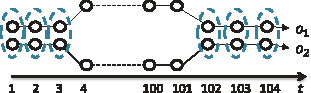
\includegraphics[width=\textwidth]{res/fig/sec-2/LooseCoupleAnomaly.pdf}
    \caption{Anomalia di connessione interrotta nel pattern \(o_1, o_2\): costituiscono un platoon valido ma le sotto-sequenze sono a 98 istanti l'una dall'altra, Fonte: \cite{DBLP:journals/pvldb/FanZWT16}}%
    \label{fig:chap-2:loose-couple-anomaly}
\end{figure}

GCMP, o General Co-Movement Pattern, è un astrazione per modellare varie tipologie di pattern di movimento.
Questa si occupa non solo di modellare i principali pattern di movimento con una tecnica univoca, ma anche di risolvere l'anomalia della connessione interrotta.

A questo proposito viene aggiunto il parametro \(g\), o gap temporale, agli altri parametri individuati nella \cref{sec:comovement-definition}.
Dati due istanti temporali \( t_1, t_2\), \(g\) rappresenta la massima distanza in termini di istanti tra questi.
Questo ulteriore vincolo permette di limitare l'anomalia della connessione interrotta: ad esempio nel caso descritto in \cref{fig:chap-2:loose-couple-anomaly} basta specificare \(g = 10\)
per scartare il pattern.

GCMP è quindi in grado di modellare pattern di movimento aventi le seguenti proprietà:

\begin{itemize}
    \item \textbf{Chiusura}.
    Dato un gruppo di oggetti \(O\) in una sequenza temporale \(T\), ogni oggetto \(o_i\) risulta vicino ad ogni altro oggetto di \(O\) ad ogni istante temporale \(t_i \in T\).
    
    \item \textbf{Importanza}.
    Definito un valore di \(m\), il numero di oggetti in \(O\) deve essere maggiore o uguale a \(m\).
    
    \item \textbf{Durata}.
    Definito un numero minimo di istanti temporali \(k\) per considerare un gruppo interessante, \(|T| \geq k \).
    
    \item \textbf{Consecutività}.
    Definito \(l\) come il valore minimo di consecutività locale, ogni sotto-sequenza continua di \(T\) deve risultare maggiore o uguale a \(l\).
    Una sequenza che rispetta questa proprietà viene detta \textit{L-consecutive}, o consecutiva rispetto a \(l\).
    
    \item \textbf{Connessione}.
    Definito \(g\) come il massimo gap tra due punti nel tempo, deve valere che \( \forall t_i \in T, d_t{(t_i, t_{i + 1}) \leq g}\).
    Una sequenza che rispetta questa proprietà viene detta \textit{G-connected}, o connessa rispetto a \(g\).
\end{itemize}

GCMP è quindi in grado di modellare tutti i pattern di co-movimento fin d'ora descritti variando i parametri come descritto nella \cref{tab:co-movement-pattern-gcmp}:

\begin{table}[H]
    \centering
   \begin{tabular}{||c c c c c||}
 \hline
     Pattern & M & K & L & G \\ [0.4ex] 
 \hline\hline
     swarm & \(m\) & \(k\) & 1 & \(\infty\) \\ 
 \hline
    closed swarm & \(m\) & \(k\) & 1 & \(\infty\) \\ 
 \hline
     convoy & \(m\) & \(k\) & \(k\) & 1 \\ 
  \hline
     group & \(m\) & 1 & \(l\) & \(\infty\) \\
  \hline
    platoon & \(m\) & \(k\) & \(l\) & \(g\) \\ 
 \hline
\end{tabular}
    \caption{Configurazioni di parametri di GCMP per la ricerca dei principali pattern di co-movimento}
    \label{tab:co-movement-pattern-gcmp}
\end{table}

SPARE (Star Partitioning and ApRiori Enumerator) è un algoritmo per la ricerca di GCMP. 
Questo framework realizza la ricerca di questi pattern suddividendo lo spazio-tempo in istanti temporali e individuando ad ogni istante quali traiettorie risultino vicine e quali no.
Successivamente genera degli itemset utilizzando gli oggetti come item e fondendoli assieme.
Intuitivamente due item saranno considerati interessanti e quindi fusi in un unico itemset se questi hanno compaiono assieme in \(k\) istanti tali che la continuità locale sia almeno di \(l\) elementi e il massimo gap non sia superiore a \(g\).
Una volta individuati questi itemset validi, l'algoritmo procede a ricercare gli itemset di almeno \(m\) elementi con le tecniche del frequent itemset mining.

Nell'ambito del lavoro di questa tesi, l'approccio di SPARE risulta interessante per due principali motivi: 
in primo luogo SPARE utilizza una tecnica di generazione e ricerca dei gruppi di movimento a metà tra il clustering e il frequent itemset mining.
Questo approccio risulta sicuramente innovativo rispetto a quanto visto fino ad ora in letteratura.
Successivamente SPARE è implementato in maniera distribuita: questo implica che possa processare enormi moli di dati in tempistiche ragionevoli.

Una volta presentate le ragioni per cui è stato scelto questo algoritmo, vengono illustrate le tre fasi di SPARE:

\begin{enumerate}
    \item \textbf{Snapshot Generation}.
    Dividendo il tempo in singoli istanti, esegue un clustering sulle posizioni spaziali di ogni oggetto ad ogni istante.
    \item \textbf{Star Partitioning}.
    Gli snaphot della fase precedente sono fusi in un grafo a stella, che successivamente viene suddiviso in ulteriori sotto-grafi sulla base
    dei nodi.
    \item \textbf{Apriori Enumerator}.
    Sfruttando una definizione custom di monotonicità basata sul tempo, esegue la trasformazione dei grafi in item.
    Successivamente conduce una ricerca di itemset frequenti e massimali, utilizzando il principio di \textit{forward closure}.
\end{enumerate}

La \cref{fig:chap-2:spare-workflow} riassume i passaggi dell'algoritmo SPARE.
Ciascuno di questi sarà analizzato nei dettagli nelle sezioni successive di questo documento.

\begin{figure}
    \centering
    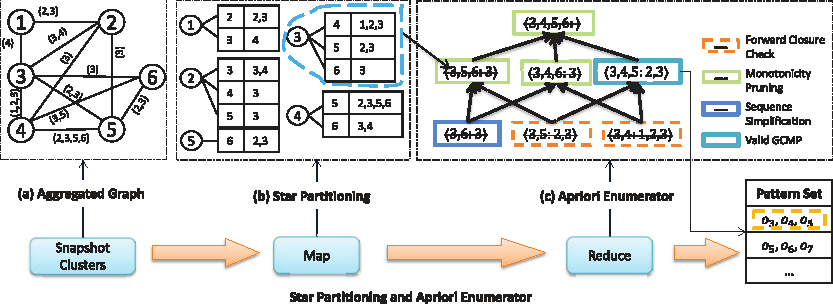
\includegraphics[width=\textwidth]{res/fig/sec-2/GCMPWorkFlow.pdf}
    \caption{Fasi di SPARE: \cite{DBLP:journals/pvldb/FanZWT16}}%
    \label{fig:chap-2:spare-workflow}
\end{figure}



